\documentclass[a4paper,12pt]{article}
\usepackage{blindtext}
\usepackage[utf8]{inputenc}
\usepackage{graphicx}

\begin{document}
\section{Functional Requirements}
In this section, we describe each feature that the system shall provide and the functional requirements for that feature. The functional requirements are the functions, inputs and outputs required for a feature or use case to be achieved. The main functions that will be used in this application in order to provide users with the described functionality are as follows:
\begin{itemize}
\item \textbf{GetLocation -} This function retrieves the GPS coordinates of a certain location. This is a critical function.
\item \textbf{GetUserLocation -} This function gives the users current location in GPS coordinates. This function is critical.
\item \textbf{SearchLocation -} This function searches for a location and if found returns its GPS coordinates. This function is critical
\item \textbf{SaveLocation -} This function saves a location. This function is important.
\item \textbf{GetDirections -} This function gets the routes from one place to another. This function is critical.
\item \textbf{GetActivity -} This function gets an activity available on campus and provides the user with its time and location. This function is nice-to-have.
\item \textbf{DetermineTraffic -} This function determines the traffic on a specified route. This function is important.
\item \textbf{ShowTraffic -} This function displays the traffic conditions to the user. This function is nice-to-have.
\item \textbf{GetPreferences -} This function gets the users preferences. This function is important.
\item \textbf{SetPreferences -} This function sets and stores the users preferences. This function is important.
\item \textbf{NotifyUser -} This function sends push notifications to the user. This function is nice-to-have.
\end{itemize}

\subsection{FindVenue Use Case}
\textbf{Description: } This use case helps the user to find a venue on campus\\
\textbf{Priority Level: } Critical\\
\textbf{Inputs:} Name of venue\\
\textbf{Outputs:} Location of inputted venue\\
\textbf{Functional Requirements: }\\
%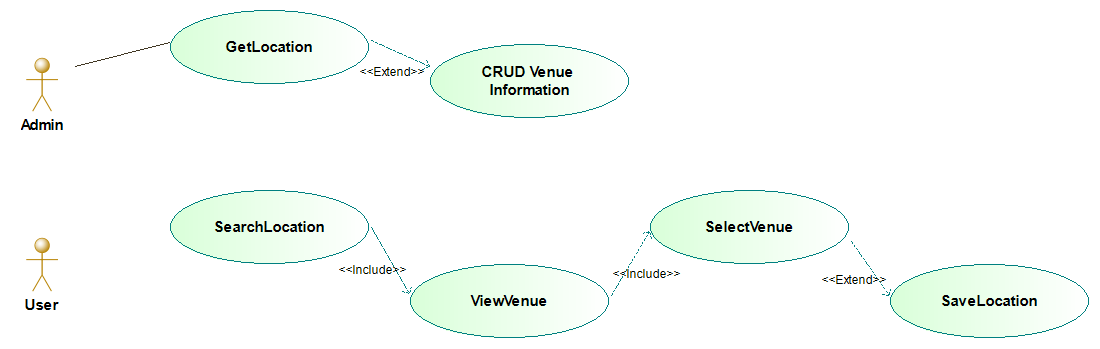
\includegraphics[width=\textwidth]{images/find_venue.jpg}

\subsection{FindService Use Case}
\textbf{Description: } This use case helps the user to find a service that is available on campus\\
\textbf{Priority Level:} Important\\
\textbf{Inputs:} A service\\
\textbf{Outputs:} Location of inputted service\\
\textbf{Functional Requirements: }\\
%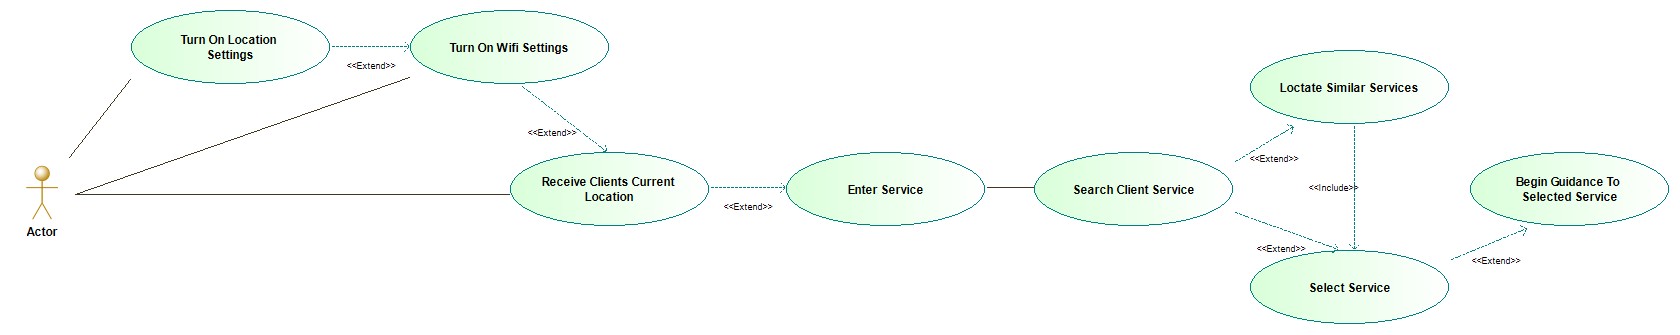
\includegraphics[width=\textwidth]{images/find_service.jpg}

\subsection{FindActivity Use Case}
\textbf{Description: } This use case helps the user to find activities at UP to participate in\\
\textbf{Priority Level: } Nice-to-Have\\
\textbf{Inputs:} Type of activity to be searched for\\
\textbf{Outputs:} Activities available with activity time and activity location\\
\textbf{Functional Requirements: }\\
%\includegraphics[width=\textwidth]{images/find_activity.jpg}

\subsection{ProvideRoute Use Case}
\textbf{Description: } This use case provides a route from a location on campus (which could be the user's current location or specified) to another location on campus (which could be specified or returned by FindVenue, FindService or FindActivity).\\
\textbf{Priority Level: } Critical\\
\textbf{Inputs:} From Where and To Where\\
\textbf{Outputs:} Route from a place to another place\\
\textbf{Functional Requirements: }\\
%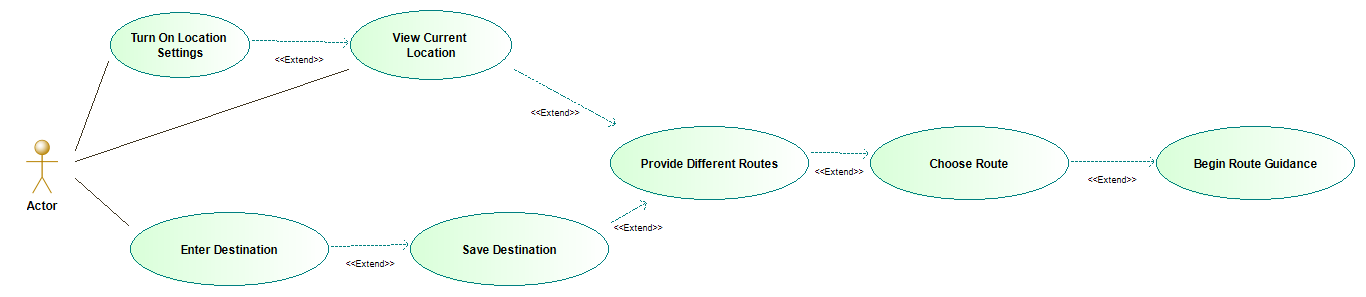
\includegraphics[width=\textwidth]{images/provide_route.jpg}

\subsection{ProvideOptimalRoute Use Case}
\textbf{Description: } This use case provides the best route from a location on campus to another location on campus. "Best" route being determined by user specified factors such as if traffic should be avoided or if the student center should be passed on the way\\
\textbf{Priority Level: } Important\\
\textbf{Inputs:} From Where, To Where and User Preferences\\
\textbf{Outputs:} Optimal route from a place to another place\\
\textbf{Functional Requirements: }\\
%\includegraphics[width=\textwidth]{images/provide_oproute.jpg}

\subsection{Traceability Matrix}
The traceability matrix visually depicts the use cases and their requirements priority in relation to one another.\\
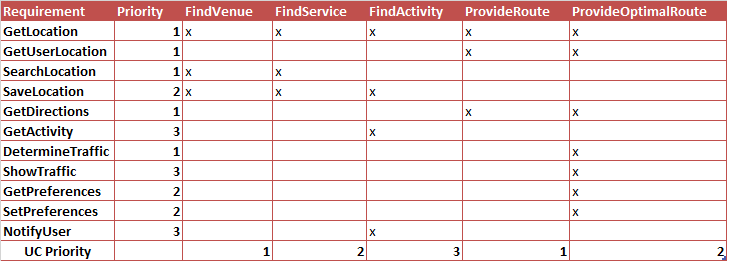
\includegraphics[width=\textwidth]{images/trmatrix.png}
\end{document}